% Document information
\documentclass{standalone} 
\usepackage[utf8]{inputenc}

\usepackage{tikz}
\usetikzlibrary{mindmap}
\pagestyle{empty}


\begin{document}
% Organises and customises nodes
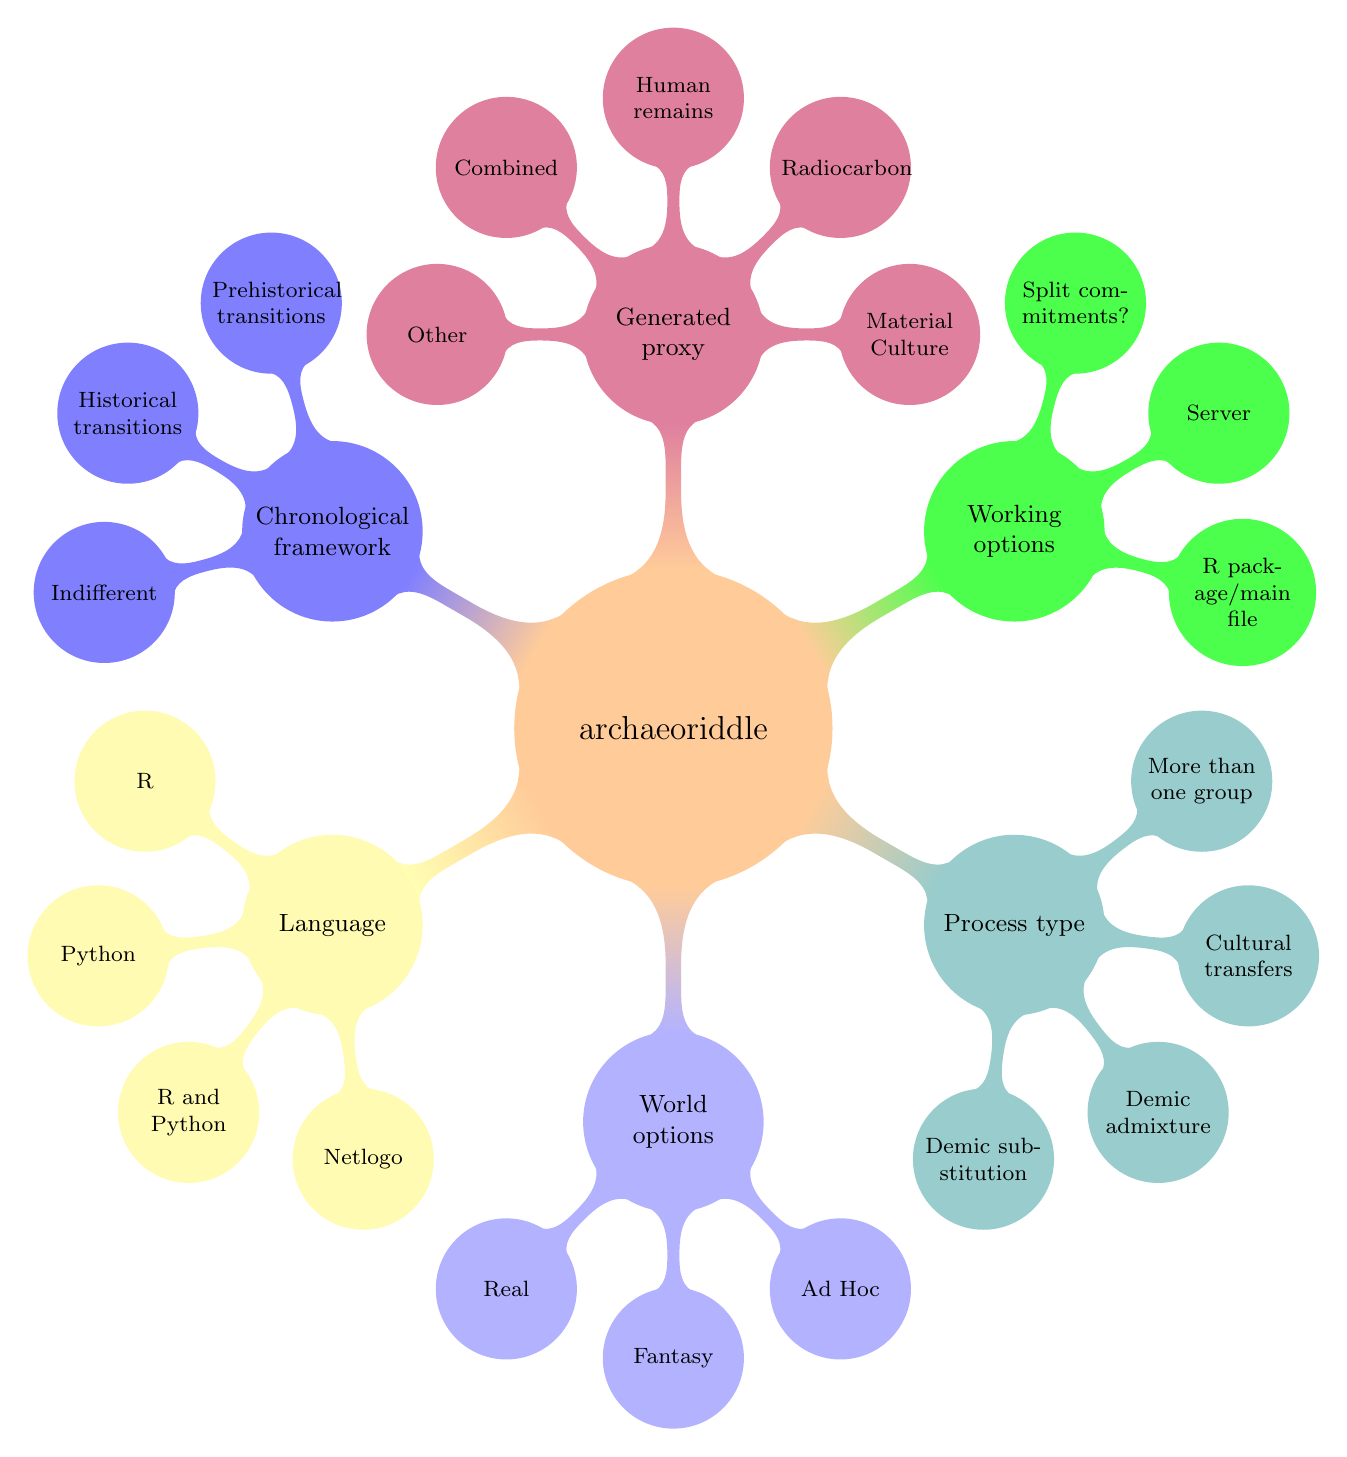
\begin{tikzpicture}[mindmap, grow cyclic, every node/.style=concept, concept color=orange!40, 
	level 1/.append style={level distance=5cm,sibling angle=60},
	level 2/.append style={level distance=3cm,sibling angle=45},]

% Create the nodes
\node{archaeoriddle}
child [concept color=yellow!30] { node {Language}
	child { node {R}}
	child { node {Python}}
	child { node {R and Python}}
	child { node {Netlogo}}
}
child [concept color=blue!30] { node {World options}
	child { node {Real}}
	child { node {Fantasy}}
	child { node {Ad Hoc}}
}
child [concept color=teal!40] { node {Process type}
	child { node {Demic substitution}}
	child { node {Demic admixture}}
	child { node {Cultural transfers}}
	child { node {More than one group}}
}
child [concept color=green!70] { node {Working options}
	child { node {R package/main file}}
	child { node {Server}}
	child { node {Split commitments?}}
}
child [concept color=purple!50] { node {Generated proxy}
	child { node {Material Culture}}
	child { node {Radiocarbon}}
	child { node {Human remains}}
	child { node {Combined}}
	child { node {Other}}
}
child [concept color=blue!50] { node {Chronological framework}
	child { node {Prehistorical transitions}}
	child { node {Historical transitions}}
	child { node {Indifferent}}
}

;

\end{tikzpicture}
\end{document}
